\documentclass[tikz, border = 5pt]{standalone}
\usepackage{tikz}

\usetikzlibrary{arrows.meta}
\usetikzlibrary{shapes.geometric}

\begin{document}

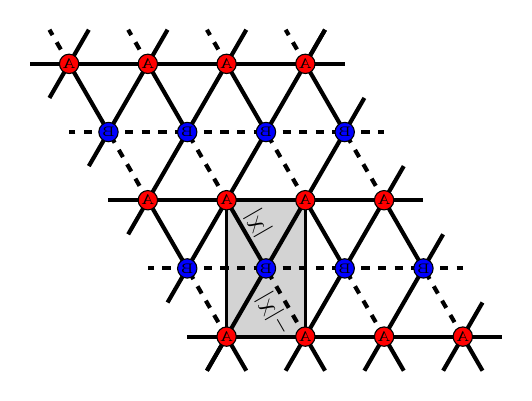
\begin{tikzpicture}[scale = 1.0]

	% model Parameters
	\def \tone{4}	% number of sites in t_1 direction
	\def \ttwo{5} 	% number of sites in t_2 direction
	\def \a{1}	% lattice paramters

	% artistic parameters
	\def \ls{dashed}
	\def \lw{1.5pt}
	\def \circsize{3.5 pt}
	\def \acolor{red}
	\def \bcolor{blue}
	\def \bzlw{1.25pt}

	% custom colors
	\definecolor{mygrey}{HTML}{d3d3d3}
	\def \bzfill{mygrey}

	% get physical coordiantes of points from i and j
	\newcommand{\getpoint}[2]{%
    		\pgfmathsetmacro{\X}{\a*(#1-0.5*#2)}%
    		\pgfmathsetmacro{\Y}{\a*#2*sqrt(3)/2}%
	}
	
% create lattice points 
	\foreach \i in {1,...,\tone} {
		\foreach \j in {1,...,\ttwo}{
			\getpoint{\i}{\j}
			\coordinate(P-\i-\j) at (\X, \Y);
		}
	}


	% draw Brillouin zone 
	\filldraw[fill = \bzfill, draw = black, line width = \bzlw] (P-1-1) -- (P-2-1) -- (P-3-3) -- (P-2-3) -- cycle;

	% draw mirrored hopping amplitude labels 
	\getpoint{2}{2}

	\pgfmathsetmacro{\Yt}{\Y + \a/sqrt(3)}
	\pgfmathsetmacro{\Xt}{\X - 0.1*\a}
	\pgfmathsetmacro{\Ymt}{\Y - \a/sqrt(3)}
	\pgfmathsetmacro{\Xmt}{\X + 0.1*\a}
	\node[rotate = -60, xscale = -1] at (\Xt, \Yt) {\footnotesize $|\chi|$};
	\node[rotate = -60, xscale = -1] at (\Xmt, \Ymt) {\footnotesize $-|\chi|$};


	% Draw nearest neighbour links for tight-binding model compatbile with pi flux pattern

	\foreach \i in {1,...,\tone}{
		\foreach \j in {1,...,\ttwo}{

			\pgfmathtruncatemacro{\parity}{mod(\j,2)}
			
			
			\ifnum \i < \tone

				% to right
				\ifnum \parity = 1
					\draw[line width = \lw] (P-\i-\j) -- (P-\the\numexpr\i+1\relax-\j);
				\else
					\draw[\ls, line width = \lw] (P-\i-\j) -- (P-\the\numexpr\i+1\relax-\j);
				\fi

				\ifnum \j < \ttwo 
					% to top right
					\draw[line width = \lw] (P-\i-\j) -- (P-\the\numexpr\i+1\relax-\the\numexpr\j+1\relax);
				\fi
			\fi


			\ifnum \j < \ttwo

				% to top left
				\ifnum \parity = 0
					\draw[line width = \lw] (P-\i-\j) -- (P-\i-\the\numexpr\j+1\relax);
				\else 
					\draw[\ls, line width = \lw] (P-\i-\j) -- (P-\i-\the\numexpr\j+1\relax);
				\fi
			\fi
		}	
	}

	% Draw half-length nearest neighbour lines outwards from outermost sides

	% Bottom edge
	\foreach \i in {1,...,\tone}{
		\draw[line width = \lw] (P-\i-1) -- ++ (0.25*\a ,{-sqrt(3)/4*\a});
		\draw[line width = \lw] (P-\i-1) -- ++ (-0.25*\a ,{-sqrt(3)/4*\a});
	}

	\pgfmathtruncatemacro{\parity}{mod(\ttwo, 2)}
	
	% Top edge
	\foreach \i in {1,...,\tone}{
		\draw[line width = \lw] (P-\i-\ttwo) -- ++ (0.25*\a ,{sqrt(3)/4*\a});

		\ifnum \parity = 0
			\draw[line width = \lw] (P-\i-\ttwo) -- ++ (-0.25*\a ,{sqrt(3)/4*\a});
		\else
			\draw[\ls, line width = \lw] (P-\i-\ttwo) -- ++ (-0.25*\a, {sqrt(3)/4*\a});
		\fi
	}

	% Left edge
	\foreach \j in {1,...,\ttwo}{

		\pgfmathtruncatemacro{\parity}{mod(\j, 2)}

		\ifnum \parity = 1
			\draw[line width = \lw] (P-1-\j) -- ++ (-0.5*\a, 0);
		\else
			\draw[\ls, line width = \lw] (P-1-\j) -- ++ (-0.5*\a, 0);
		\fi

		\draw[line width = \lw] (P-1-\j) -- ++ (-0.25*\a, {-sqrt(3)*\a/4});
	}

	% Right edge
	\foreach \j in {1,...,\ttwo}{

		\pgfmathtruncatemacro{\parity}{mod(\j,2)}

		\ifnum \parity = 1
			\draw[line width = \lw] (P-\tone-\j) -- ++ (0.5*\a, 0);
		\else
			\draw[\ls, line width = \lw] (P-\tone-\j) -- ++ (0.5*\a, 0);
		\fi

		\draw[line width = \lw] (P-\tone-\j) -- ++ (0.25*\a, {sqrt(3)*\a/4});
	}

	% draw bubbles at lattice points with alternating point

	\foreach \i in {1,...,\tone}{
		\foreach \j in {1,...,\ttwo}{
			
			\pgfmathtruncatemacro{\parity}{mod(\j, 2)}

			\ifnum \parity = 1
				\filldraw[draw=black, fill=\acolor]  (P-\i-\j) circle (\circsize) node[xscale = -1] {\tiny A};
			\else
				\filldraw[draw=black, fill = \bcolor] (P-\i-\j) circle (\circsize) node[xscale = -1] {\tiny B};
			\fi
		}
	}


\end{tikzpicture}

\end{document}
